\chapter{Frequency Modulated Continuous Wave Radar}
As the name Frequency Modulated Continuous Wave (FMCW) implies, a FMCW radar is
a continuous time system which transmits and receives a periodic signal whose 
frequency has been modulated. As a periodic signal, the transmitted signal has
the complex form (with unit-normalized amplitude)
\begin{equation}
	\label{eq:complex-sinusoid}
	p(t) = e^{j2\pi f(t)t}.
\end{equation}
The typical frequency modulation used in FMCW radar systems is the sawtooth
modulation, given by
\cite{iovescufundamentals, wang2008digital}
\begin{equation}
	\label{eq:sawtooth}
	f(t) = f_c + \alpha t, \quad 0<t<T_c 
\end{equation}
where $\alpha > 0$ is the chirp-rate  $\frac{df}{dt}$, $f_c$ is the base
carrier frequency (e.g. 77 GHz), and $T_c$ is the period of the chirp. The
maximum frequency of each chirp is thus
\begin{equation}
	f_{max} \triangleq f_c + \alpha T_c,
\end{equation}
and the bandwidth $B$ of the signal is
\begin{equation}
	B = f_{max} - f_c = \alpha T_c.
\end{equation}

Combining the sawtooth frequency modulation (\ref{eq:sawtooth}) with the complex
sinusoid (\ref{eq:complex-sinusoid}), we get
the transmitted (TX) signal as
\begin{equation}
	p(t) = e^{j(2\pi f_c t+ \pi \alpha t^2)}.
\end{equation}

\begin{figure}[h]
	\centering
	\begin{subfigure}[b]{0.8\textwidth}
		\begin{tikzpicture}
			\begin{axis}[
			axis x line = bottom,
			axis y line = left,
			xlabel = $t$,
			ylabel=$f(t)$,
			xmin=0, xmax=8,
			ymin=0, ymax=3.2,
			xtick=\empty,
			ytick=\empty,
			xlabel near ticks,
			ylabel near ticks,
			extra x ticks={4,8},
			extra x tick labels={$T_c$, $2T_c$},
			extra y ticks={0, 1, 3},
			extra y tick labels={$0$, $f_c$, $f_{max}$},
			]
			\draw 
				(axis cs:1.5, 1.75)
				-| (axis cs:2, 2)
				node [near end, right]
				{$\alpha$};
			\addplot [
			domain=0:8,
			samples=100,
			color=black,
			]
			{(1 + 0.5*x)*(x<4)+(1+0.5*(x-4))*(x>4)};
			\end{axis}
		\end{tikzpicture}
		\label{fig:sawtooth}
		\caption{Example of sawtooth frequency modulation}
	\end{subfigure}
	\begin{subfigure}[b]{0.8\textwidth}
		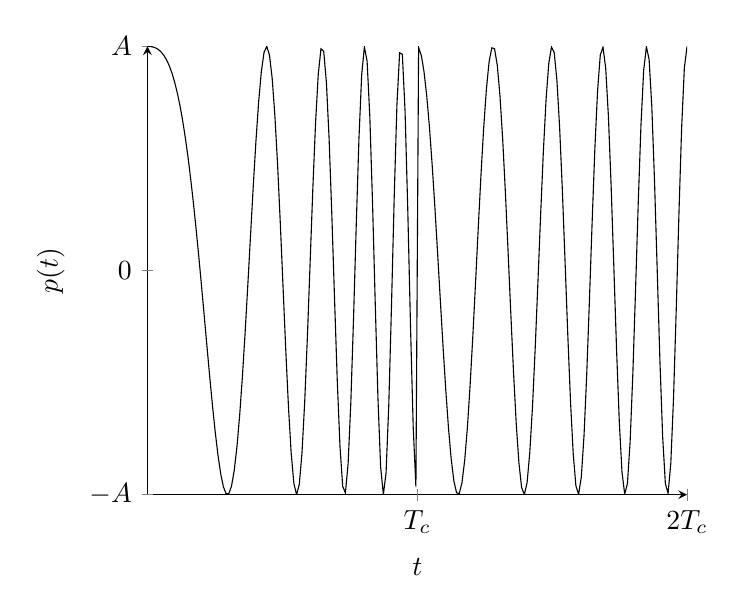
\begin{tikzpicture}
			\begin{axis}[
			axis x line = bottom,
			axis y line = left,
			xlabel = $t$,
			ylabel=$p(t)$,
			xmin=0, xmax=8,
			ymin=-1, ymax=1,
			xtick=\empty,
			ytick=\empty,
			xlabel near ticks,
			ylabel near ticks,
			extra x ticks={4,8},
			extra x tick labels={$T_c$, $2T_c$},
			extra y ticks={-1, 0, 1},
			extra y tick labels={$-A$, $0$, $A$},
			]
			\addplot [
			domain=0:8,
			samples=200,
			color=black,
			]
			{cos(deg(2*pi*((0.125 + 0.25*x)*(x<4)+(0.25+0.125*(x-4))*(x>4))*x)};
			\end{axis}
		\end{tikzpicture}
		\label{fig:pulse}
		\caption{Example of TX signal $p(t)$}
	\end{subfigure}
\end{figure}

\section{Range Measurement}
Consider a target at a distance $d$ from the radar, such that the transmitted
(RX) signal reflects off the target and returns to the radar. This received signal
will be a time delayed version of the TX signal, where the time delay $\tau$ is
given by
\begin{equation}
	\tau = \frac{2d}{c}
\end{equation}
where $c$ is the speed of light. The RX signal thus has the form
\begin{equation}
	p(t-\tau)=e^{j(2\pi f_c (t-\tau) + \pi\alpha (t-\tau)^2)}.
\end{equation}

\begin{figure}[h]
	\centering
	\begin{tikzpicture}
		\begin{axis}[
		axis x line = bottom,
		axis y line = left,
		xlabel = $t$,
		ylabel=$f(t)$,
		xmin=0, xmax=8,
		ymin=0, ymax=3.2,
		xtick=\empty,
		ytick=\empty,
		xlabel near ticks,
		ylabel near ticks,
		extra x ticks={1,4,8},
		extra x tick labels={$\tau$,$T_c$, $2T_c$},
		extra y ticks={0, 1, 1.5, 3},
		extra y tick labels={$0$, $f_c$, $f_b$, $f_{max}$},
		]
		\draw[dashed] (axis cs:0, 1.5) -| (axis cs:1, 0);
			
		\addplot [
		domain=0:8,
		samples=100,
		color=black,
		]
		{(1 + 0.5*x)*(x<4)+(1+0.5*(x-4))*(x>4)};
		\addplot [
		domain=0:8,
		samples=100,
		color=red,
		]
		{(x<1)*1 + (1+0.5*(x-1))*(x>1)*(x<5) + (1+0.5*(x-5))*(x>5)};
		\end{axis}
	\end{tikzpicture}
	\label{fig:received}
	\caption{Frequency of RX signal (delayed by time $\tau$)}
\end{figure}

To recover $\tau$, and subsequently $d$, we define a new dechirped signal $r(t)$
as the product of the transmitted signal with the complex conjugate of the
received signal
\begin{align}
	r(t) &\triangleq p(t)p^*(t-\tau) \\
	&= e^{j(2\pi f_c t + \pi \alpha t^2)}e^{-j[2\pi f_c (t-\tau) + \pi\alpha (t-\tau)^2 ]} \\
	&= e^{j(2\pi f_c \tau - \pi \alpha \tau^2)}e^{j2\pi\alpha\tau t}.\label{eq:range}
\end{align}
Note, the first exponential in (\ref{eq:range}) only depends on $\tau$, so it is
a constant phase term. However, the second term varies according to a constant
frequency (named the beat frequency) $f_b$
\begin{equation}
	f_b \triangleq \alpha \tau.
\end{equation}
The maximum beat frequency occurs when $\tau = T_c$, as any $\tau > T_c$ will
appear as $\tau^*$
\begin{equation}
	\tau^* = \tau - T_c, \quad \tau > T_c
\end{equation}
and thus the recovered distance $d^*$ will be less than the true range the
target is from the radar. From this, we can get our maximum recoverable distance
for a given chirp period
\begin{equation}
	d_{max} = \frac{c T_c}{2}.
\end{equation}
To recover the beat frequency $f_b$ from the dechirped signal, $r(t)$, we can
simply use the Fourier Transform to get
\begin{align}
	R(f) &= \int_{-\infty}^{\infty} r(t) e^{-j2 \pi ft} dt\\
	&= \int_{-\infty}^{\infty} e^{j(2\pi f_c \tau - \pi \alpha \tau^2)}e^{j2\pi\alpha\tau t} e^{-j2\pi ft}dt\\
	&= e^{j(2\pi f_c \tau - \pi \alpha
	\tau^2)}\int_{-\infty}^{\infty}e^{-j2\pi(f - \alpha\tau ) t} dt\\
	&= e^{j(2\pi f_c \tau - \pi \alpha \tau^2)}\delta (f - \alpha \tau),
\end{align}
where $\delta(f)$ is the Dirac Delta function.


